\section{Recurrent weight estimation}

We implement the recurrent weight estimation as a variational problem, i.e. define: \begin{equation}\label{eq-criterion} {\bf W} = \mbox{arg min}_{{\bf W}} \mbox{min}_{\bf x} \mbox{max}_{\bf \varepsilon} \; {\cal L}({\bf W} , {\bf x}, {\bf \varepsilon}) ,\end{equation}
for adjustable network parameters or weights ${\bf W}$, given state values ${\bf x}$ and auxilary variables ${\bf \varepsilon}$, writing:
\eqline{\begin{array}{rlll} {\cal L}({\bf W} , {\bf x}, {\bf \varepsilon}) \deq
& \rho(\cdots, x_n(t), \cdots)  & \mbox{\small desired values} \\
+& \sum_{nt} \varepsilon_{nt} \, (\tilde{x}_n(t) - x_n(t)) & \mbox{\small network dynamic constraint} \\
+& {\cal R}({\bf W}) & \mbox{\small regularization} \\
\end{array}}
where $\tilde{x}_n(t)$ is a shortcut for equation~(\ref{eq-recurrent}):
\eqline{\left\{ \begin{array}{rcl}
\tilde{x}_n(t) &\deq& \Phi_{n0t}\left(\cdots, x_{n'}(t'), \cdots, i_{m}(s), \cdots\right) \\
 &+& \sum_{d = 1}^{D_{n}} W_{nd} \, \Phi_{ndt}\left(\cdots, x_{n'}(t'), \cdots, i_{m}(s), \cdots\right)
\end{array} \right.}
while $\varepsilon_{nt}$ are Lagrange multipliers, and in most of the cases\footnote{More precisely, here, in the deterministic case, a simple additive criterion is used, while this is not the case for statistical criterion, as further discussed in appendix~\ref{application} and~\ref{stochastic}.} we use:
\eqline{\rho(\cdots, x_n(t), \cdots) \deq \sum_{nt} \rho_{nt}(x_n(t)).}

Here $\rho()$ is a cost-function (acting both as supervised or unsupervised variational term) and ${\cal R}({\bf W})$ some regularization term, as made explicit in Appendix~\ref{application}. The cost function includes both the term attached to the data, i.e., the fact that output values have a desired values, and regularization. These ingredients can be used to get the approximate desired output, yield sparse estimation, reduce artifact influence, obtain activity orthogonality, etc (see Appendix~\ref{application} for details).

In a nutshell, $\rho()$ and ${\cal R}$ allows one to specify the estimation problem, as a function of the unknows ${\bf W}$, ${\bf x}$ and ${\bf \varepsilon}$. Stating the estimation this way, leads us to a simplified form of the Pontryagin's minimum principle, well-known in control theory \cite{astrom:83}, and reviwed in the next section. In short, the effective related solution is derived from the normal equations of the proposed criterion.

This formulation is not new and has been formalized, by, e.g. \cite{cun_theoretical_1988}. Here we restate it at a higher level of generality, with two new aspects: (i) making explicit the role of the Lagrange multiplier (also called adjoint state in this context) for hidden units and (ii) proposing a 2nd order local estimation mechanism. The relation with other recurrent weights estimation methods is discussed in Appendix~\ref{backpropag}.

Applying standard derivations, the criterion gradient writes:
\eqline{\begin{array}{rcll}
\partial_{\varepsilon_{nt}} \, {\cal L} &=& \tilde{x}_n(t) - x_n(t) \\
&&\\
\partial_{x_{n'}(t')} \, {\cal L} &=&  
-\varepsilon_{n't'} + \rho'_{n't'} + \sum_{nt, \begin{array}{c} t' < t \leq t' + R \\ or\; t' = t, n < n'\end{array}} \beta_{nt}^{n't'} \, \varepsilon_{nt} \\
&&\\
\partial_{W_{nd}} \, {\cal L}  &=& \sum_{n'', W_{n''d} = W_{nd}} \sum_t \phi_{n''dt} \, \varepsilon_{n''t} + \partial_{W_{nd}} \, {\cal R} \\
\end{array}}
writing : 
{\small \eqline{\left\{ \begin{array}{rclcl}
\rho'_{nt} &\deq& \partial_{x_n(t)} \rho(\cdots, x_n(t), \cdots) \\
&\\
\phi_{ndt} &\deq& \Phi_{ndt}\left(\cdots, x_{n'}(t'), \cdots, i_{m}(s), \cdots\right) &=& \partial_{W_{nd}} \tilde{x}_n(t)\\
&\\
\beta_{nt}^{n't'} &\deq& \partial_{x_{n'}(t')} \phi_{n0t} + \sum_{d = 1}^{D_{n}} W_{nd} \, \partial_{x_{n'}(t')} \phi_{ndt} &=& \partial_{x_{n'}(t')} \tilde{x}_n(t) \\
&\\
\end{array} \right.}}

The sum $\sum_{nt, \begin{array}{c} t' < t \leq t' + R \;or\; t' = t, n < n'\end{array}}$ encounters for previous values and subsequent node values. This sum includes terms with $\beta_{nt}^{n't'} \neq 0$, i.e. terms for which there is a recurrent connection from the node of index $n$ at time $t$ onto the node of index $n'$ at time $t'$. We simply write $\sum_{nt}$ in the sequel, without any risk of ambiguity.

The sum $\sum_{n'', W_{n''d} = W_{nd}}$ encounters for weight sharing, i.e., the fact that weights from different units may be constrained to have the same value. We will simply write $\sum_{n''}$ in the sequel, without any risk of ambiguity.

Let us now review and discuss how we can implement such a minimization.

\subsection*{The minimization steps}

\subsubsection*{Forward simulation}

The equation $\partial_{\varepsilon_{nt}} {\cal L} = 0$ yields $x_n(t) = \tilde{x}_n(t)$. This simply means that $x_n(t)$ is iven by the network equation, i.e., equation~(\ref{eq-recurrent}). Since $\tilde{x}_n(t)$ depends on previous values at time $t' < t$, it provides a closed-form formula to evaluate $x_n(t)$ from the beginning to the end. This simply corresponds to the fact that the dynamic is simulated. This step depends on the weights $W_{nd}$ but not on the Lagrange multipliers $\varepsilon_{nt}$. At the end of the step the equality $\partial_{\varepsilon_{nt}} \, {\cal L} = 0$ is obtained, and the criterion value itself does not depends on $\varepsilon$ since the constraints are verified. As a consequence, the criterion value ${\cal L}$ can be calculated during this step.

The forward simulation complexity corresponds to the network simulation and is of order $O(N D T)$ with a memory resources of $O(N T)$ since we must buffer the calculated output,  for subsequent calculations.

\subsubsection*{Backward tuning}

The equation $\partial_{x_{n'}(t')} {\cal L}  = 0$ also provides a closed-form formula to evaluate $\varepsilon_{n't'}$ as a linear function of subsequent values $\varepsilon_{nt}, t > t'$, so that the calculation is to be done from the last time $t = T-1$ backward to the first time $t = 0$:
\begin{equation} \label{backward-tuning}
\varepsilon_{n't'} = \rho'_{n't'} + \sum_{nt} \beta_{nt}^{n't'} \, \varepsilon_{nt}.
\end{equation}

This is the key feature of such a variational approach, allowing backward tuning, i.e., take into account the fact that adjusting the system parameters for a node $n$ at time $t$ is interdependent with the state of subsequent computations.

This makes the key difference with respect to usual approaches based on gradient back-propagation: Here the output error is back-propagated. 
This calculation may be recognized as a kind of back-propagation, but it is mathematically different.
This method is thus quite different from back-propagation-though-time recurrent network or other standard alternatives. 


As mentioned by \cite{cun_theoretical_1988}, $\beta_{nt}^{n't'}$ is nothing more than the first order approximation of the backward dynamics, technically the product of the weight matrix with the system Jacobian.

This backward computation is local to a given unit in the sense that only efferent units (i.e., units this unit is connected to) are involved in the computation of the related Lagrange parameter. This step depends on both weights and output values, and the equality $\partial_{\varepsilon_{nt}} \, {\cal L} = 0$ is obtained at the end.

The backward tuning step has the same order of magnitude in terms of calculation $O(N D T)$  and memory resources of $O(N T)$ (in fact of $O(N R)$, because the obtained result may be immediately re-used to compute the 2nd and 1st order weight adjustment quantities, discussed in the sequel). 

\paragraph{\em Parameter interpretation.}

We obtain, from equation~(\ref{backward-tuning}) after some algebra $\varepsilon_{n't'} = \sum_{nt} B_{n't'}^{nt} \, \rho'_{nt}$, with finite summations and for some quantities $B_{n't'}^{nt}$ (not made explicit here) which are unary coefficient polynomial in $\beta_{nt}^{n't'}$. This made explicit the fact $\varepsilon_{n't'}$ is a linear function of subsequent errors, i.e., a backward tuning error.

If $\beta_{nt}^{n't'} = 0$, there is no dependency of ${x}_n(t)$ on ${x}_{n'}(t')$, i.e. no recurrent connection. If the unit has no recurrent connection, i.e. is a not a function of other units, then $\varepsilon_{n't'} = \rho'_{nt}$ is simply related to the cost function derivative. In the least-square case (i.e. if $\rho_{nt} = \frac{1}{2} \, (x_{nt} - \bar{o}_{nt})^2$), then $\rho'_{nt} = x_{nt} - \bar{o}_{nt}$ is the output error.

\paragraph{\em Real-time aspects.}

Such a formulation is definitely not ``real-time'', since we ``go back in time''. It is however, the only solution for hidden layers to be tuned, since the output adjustment is a function of hidden activity in the past, the estimation must thus take future information into account in order to properly adapat.

However, in a real-time paradigm, it must be noted that each computation is also local in {\em time}: It only depends on values in a ``near future'' within a time range equal to the system time range. In other words, at a given time we obtain the value with a lag equal to system time-range. It is an interesting perspective of this work to explore if, considering only a bounded window-time may provide numerically relevant values for on-the-fly backward tuning.

\paragraph{\em Numerical stability.}

This back-propagation of tuning error, may suffer from the same curse than back-propagation of gradient, as reviewed in e.g., \cite{Hochreiter:1997}: Either error explosion (if $|\beta_{nt}^{n't'}| > 1$), or error extinction (if $|\beta_{nt}^{n't'}| < 1$). Based on this remark, the key idea of LSTM \cite{Hochreiter:1997} is to consider memory carousel (detailled in Appendix~\ref{generality}) to guaranty $\left|\beta_{nt}^{n't'}\right| \simeq 1$ and thus a stable back-propagation for at least some recurrent link, but this means that the designer of the network architecture has to consider such predefined units, which is a strong constraint.

In our case, since all kernels are contracting with $\max|\partial_{x_{n'}(t')} \phi_{ndt}| = 1$ we are in a situation where the a-priory numerical conditioning is optimal. We also have the bound, writing $\beta_{max} \deq \max_{nt} |\beta_{nt}^{n't'}|$ :
\eqline{0 \leq \left|\beta_{nt}^{n't'}\right| \leq \beta_{max} \leq 1 + \sum_d |W_{nd}|}
without any thinner inequality in the general case. This means that we ``must'' accept error potential explosion as soon as the weights values are not below one, which can not be a manageable constraint.

\begin{figure}[!ht]
  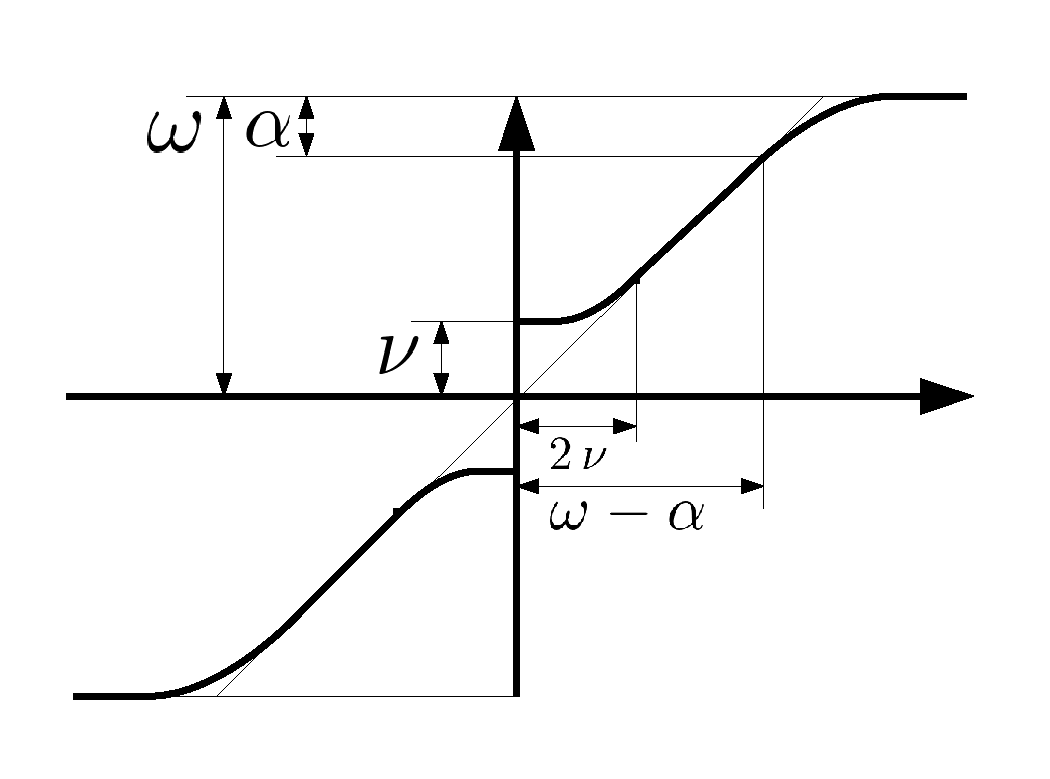
\includegraphics[width=0.8\textwidth]{img/backward-guard}
  \caption{The backward guard profile, defined in~(\ref{eq-g}), with a bias for tiny values and a saturation for huge values.}
  \label{backward-guard}
\end{figure}

To avoid backward explosion or extinction, we are going to introduce another heuristic: We are going to {\em bias} the backward error given in equation~(\ref{backward-tuning}). We define:
\begin{equation} \label{kappa}
\varepsilon_{n't'} \simeq \rho'_{nt} + g\left(\sum_{nt} \beta_{nt}^{n't'} \, \varepsilon_{nt}\right),
\end{equation} considering a function $g(u)$, shown in Fig.~\ref{backward-guard}. It is the identity function except for small vanishing values that are raised using a simple quadratic profile, an huge values saturated by an exponential profile, and providing a continuously derivable function. This design choice writes, for fixed meta-parameters $\omega, \alpha, \nu$:
\begin{equation}\label{eq-g} g(u) \deq sg(u) \, \left\{ \begin{array}{cl} 
\omega - \alpha \, e^{-\frac{|u| - \omega}{\alpha} - 1} & \omega - \alpha \leq |u| \\
|u| & 2 \, \nu \leq |u| \leq \omega - \alpha \\
\nu + \frac{u^2}{4 \, \nu} & |u| \leq 2 \, \nu, \\
\end{array} \right.\end{equation}
where $sg()$ is the sign function. To fix these meta-parameters we consider the order of magnitude of the output error:
\eqline{\bar{\rho'} \deq \frac{\sum_{nt, \rho'_{nt} \neq 0} \rho'_{nt}}{\sum_{nt, \rho'_{nt} \neq 0} 1}, }
and a reasonable choice to preserve the numerical conditioning is $\nu = 10^{-6} \, \bar{\rho'}$ and $\omega = 10^{6} \, \bar{\rho'}$, with e.g., $\alpha = 10^{-3} \, \omega$. They are very likely not to be adjusted because they only correspond to order of magnitude of numerical calculation. We have observed that using double precision floating numbers on a standard processor for such kind of calculations corresponds to such rough numbers.

\subsubsection*{The 2nd order unit weight adjustment}

We now have to estimate the weights ${\bf W}$ and are left with the last normal equation $\partial_{W_{nd}}\, {\cal L} = 0$ which is not an explicit function of the weights. On track is to use the gradient to minimize the criterion using a 1st order method, this is discussed in the next sub-section. Interesting enough is the fact that we can also propose a 2nd order method as made explicit and derived now. In other words, we reintroduce a linear estimation of the weights assuming that the criterion is locally quadratic.

We thus propose to use the following 2nd order weight adjustment:
\begin{equation} \label{2nd-order}
\sum_{n''} b_{n'',\,d} = \sum_{n''} \sum_{d'=1}^{D_{n}} A_{n'',\,d\;d'} \, W_{n''d'}
\end{equation}
writing, for some $\kappa_{nt}$: 
\eqline{\left\{ \begin{array}{rcl}
b_{n,\,d} &\deq& \sum_t \phi_{ndt} \, \left( \varepsilon_{nt}  + \kappa_{nt} \, \left(\hat{x}_n(t) - \phi_{n0t} \right) \right)  + \partial_{W_{nd}} \, {\cal R}(\hat{\bf W}),  \\
&\\
A_{n,\,d\;d'} &\deq& \sum_t \kappa_{nt} \, \phi_{ndt} \, \phi_{nd't},  \\
\end{array} \right.}
where:
\\- $\hat{x}_n(t)$ is best present estimate of $x_n(t)$,
\\- $\hat{\bf W}$ is the best estimate of ${\bf W}$ at the present step.

This allows us to obtain a new weight value ${\bf W}$ solving a linear system of equation for each unit and the closest solution\footnote{{\bf Minimal distance pseudo-inverse.} We consider: 
\eqline{\min_{{\bf W}} ||{\bf W} - \hat{\bf W}||, {\bf b} = {\bf A} \, \hat{\bf W}}
which is directly obtained using the singular value decomposition of the symmetric matrix ${\bf A} = {\bf U} \, {\bf S} \, {\bf U}^T$:
\eqline{{\bf W} = \hat{\bf W} + {\bf A}^\dagger \, ({\bf b} - {\bf A} \, \hat{\bf W}),} 
where ${\bf A}^\dagger$ is the pseudo-inverse of ${\bf A}$.\hr} with respect to $\hat{\bf W}$ is considered.

The derivation\footnote{\label{improvingkappa}{\bf Deriving the 2nd order adjustment form.} Let us omit the ${\cal R}()$ term and avoid considering weight sharing in this derivation, in order to lighten the notations.  The complete derivation would have obviously led to similar results.

Given a desired value estimate $\hat{x}_n(t)$, without loss of generality we can write, for some general quantity $\kappa_{nt}({\bf W} , {\bf x}, {\bf \varepsilon})$:
\eqline{{\cal L}({\bf W} , {\bf x}, {\bf \varepsilon}) = \sum_{nt} \frac{\kappa_{nt}({\bf W} , {\bf x}, {\bf \varepsilon})}{2} \, \left(\tilde{x}_n(t) - \hat{x}_n(t)\right)^2,}
yielding for $\partial_{W_{nd}} {\cal L}$:
\eqline{\sum_{t} \kappa_{nt}({\bf W} , {\bf x}, {\bf \varepsilon})  \, \phi_{ndt} \, (\tilde{x}_n(t) - \hat{x}_n(t)) + \sum_{t} \partial_{W_{nd}} \kappa_{nt}({\bf W} , {\bf x}, {\bf \varepsilon}) \, (\tilde{x}_n(t) - \hat{x}_n(t))^2 / 2 = \sum_t \phi_{ndt} \, \varepsilon_{nt}.} 
For a simple least-square criterion,  $\kappa_{nt} \in \{0, 1\}$ depending on the fact that the desired output $\bar{o}_n(t)$ is defined or not, and it is straight-forward to verify in this particular case that the proposed 2nd order weight adjustment reduces to an exact linear system of equation, in the absence of recurrent links of the given unit, since $\phi_{ndt}$ is only function of the input. Otherwise, $\phi_{ndt}$ is also a function of both the network unknown output and hidden node values.
\\ (i) In our case the output and backward error estimation is $\varepsilon_{nt}$, i.e., we can set $\hat{x}_n(t) \deq \tilde{x}_n(t) - \varepsilon_{nt}$ as a corrected value of the last estimate $\tilde{x}_n(t)$. Given this hypothesis, it is obvious to verify that $\kappa_{nt}({\bf W} , {\bf x}, {\bf \varepsilon}) = 1$ verifies the equation.
% dsolve({kappa(w) * phi * (phi * w - psi) + D(kappa)(w) * (phi * w - psi)^2 / 2 = phi * epsilon}, {kappa(w)}); 
\\ (ii) A step further, for a general value $\hat{x}_n(t)$, a sufficient condition now writes:
\eqline{\kappa_{nt}({\bf W} , {\bf x}, {\bf \varepsilon}) = 2 \, \varepsilon_{nt} / (\tilde{x}_n(t) - \hat{x}_n(t)),}
thus $k_nt$ is proportional to $\varepsilon_{nt}$ and must decrease with the prediction error increase.
Considering the case (i), it is straightforward to verify that if $\kappa_{nt}$ is constant, and assuming $\hat{x}_n(t)$ is fixed, we obtain the related least-square linear equations given in~(\ref{2nd-order}).
\hr}.

More sophisticated estimated values can be considered\footnote{\label{improvingstate}{\bf Improving the best estimate of the state value.} The best estimate of the state value $\hat{x}_n(t)$ given output values $\bar{o}_{n_0}(t)$ is not obtained by the simulation since $\hat{x}_{n_0}(t) \neq \bar{o}_{n_0}(t)$.

If we consider the value obtained by simulation (i.e., the $\tilde{x}_n(t)$ values), corrected by the error estimate thus $\hat{x}_n(t) = \tilde{x}_n(t) - \varepsilon_{nt}$, for a least-square criterion, it is easy to verify that this yields $\hat{x}_{n_0}(t) = \bar{o}_{n_0}(t)$. 

For output node value the $\bar{o}_n(t)$ desired value could be enforced, limiting recurrent perturbation and yielding $\phi_{ndt}$ values closed to the ideal value, which is interesting in reverse-engineering estimation, i.e. when an exact solution is expected \cite{rostro-gonzalez-cessac-etal:10}, whereas a bias in the estimation is otherwise expected, since hidden units simulated values and output values are not coherent.

A step further, we propose to retro-propagate the output value through the recurrent network, given weights values $\hat{\bf W}$, i.e., estimate:
\eqline{\hat{x}_n(t) = \mbox{arg min}_{{x}_n(t)} {\cal M}, \;\;\; {\cal M} = \frac{1}{2} \sum_{n, n \geq N_0 \; t} ({x}_n(t) - \Phi_{nt}\left(\cdots, {x}_{n'}(t'), \cdots\right))^2, {x}_{n_0}(t) = \bar{o}_n(t)}
in words find the state values for which the simulation errors yielding the desired output are minimal. Considering the normal equation $\partial_{x_{n'}(t')} {\cal M} = 0$ we obtain the recurrent equation:
\eqline{\hat{x}^k_{n'}(t') = \left\{\begin{array}{ll}
 \bar{o}_{n'}(t') & n' < N_0 \\
 \Phi_{nt}\left(\cdots, \hat{x}^{k-1}_{n'}(t'), \cdots\right) - \sum_{nt} \beta_{nt}^{n't'} \, (\hat{x}^{k-1}_{n}(t) - \Phi_{nt}\left(\cdots, \hat{x}^{k-1}_{n'}(t'), \cdots\right)) & N_0 \leq n', \end{array}\right.}
i.e., the simulation value is corrected considering a backward propagation of the simulation error.

In fact, it is simple to verify that we implicitly solve a system of $N\,T$ equations in $N\,T$ unknowns, the numerical scheme allowing to converge to a solution closed to the simulation values. This has been numerically verified in the experimentation.

It has been implemented as an option in the software in order to help improving the convergence of the recurrent weight adjustment. \hr}.

The weight adjustment is local to each unit, providing a true distributed mechanism  (unless if weight sharing is considered, because weights from different units are to be estimated together using the proposed equations). This corresponds to a 2nd order minimization scheme. Each step requires $O(N (D T + D^3)$- operation, solving a linear system of equations. The $O(N\,D^3)$ is critical if the network connectivity $D$ is high, and this does not depend on the linear system resolution method (e.g., SVD or Cholesky decomposition). The implemented method stands on the singular-value-decomposition of the matrices ${\bf A}_n$.

This offers an alternative to 2nd order adjustment methods such as \cite{martens_learning_2016} or other methods reviewed in \cite{Goodfellow2016Deep}.

In fact, a standard 2nd order adjustment can be derived in closed form\footnote{{\bf Calculating the standard 2nd order weight adjustment.} The criterion Hessian, omitting the regularization term and weight sharing to lighten the notations, writes:
\eqline{\left\{\begin{array}{rclcl}
\partial_{\varepsilon_{nt} \varepsilon_{n't'}} \, {\cal L} &=& 0 \\
\partial_{x_{n'}(t') \varepsilon_{nt}} \, {\cal L} &=& \beta_{nt}^{n't'} \\
\partial_{W_{nd} \varepsilon_{n't'}} \, {\cal L} &=& \delta_{n=n'} \, \phi_{ndt'} \\
\partial_{x_{n'}(t') x_{n''}(t'')} \, {\cal L} &=&  H^{nt}_{n't'n''t''} &\deq& \sum_{nt} \partial_{x_{n'}(t') x_{n''}(t'')} \left(\rho() + \phi_{n0t} + \sum_{d = 1}^{D_{n}} W_{nd} \, \phi_{ndt}\right) \\
\partial_{W_{nd} x_{n'}(t')} \, {\cal L} &=&  J^{nd}_{n't'} &\deq& \sum_t \varepsilon_{nt} \, \partial_{x_{n'}(t')} \phi_{ndt} \\
\partial_{W_{nd} W_{n'd'}} \, {\cal L} &=& 0, \\
\end{array}\right.}
writing $\beta_{nt}^{nt} \deq -1$. 

The 1st remark is that $H^{nt}_{n't'n''t''}$ and $J^{nd}_{n't'}$ are not local to one node, whereas the summation involves all nodes connected to the given one. Furthermore if $\rho()$ is not a sum of local terms but a statistical criterion $H^{nt}_{n't'n''t''}$ is a function of the whole network.

Then the standard 2nd order scheme $0 \simeq \nabla {\cal L} + \nabla^2 {\cal L} \, \delta({\bf W}, {\bf x}, {\bf \varepsilon})$ writes in our case where $\partial_{\varepsilon_{nt}} {\cal L} = \partial_{x_{n'}(t')} {\cal L} = 0$:
\eqline{\left\{\begin{array}{rccrccrccl}
&&&\sum_{n't'} \beta_{nt}^{n't'} & \delta x_{n'}(t') &+& \sum_d \phi_{ndt} & \delta W_{nd}  &\simeq& 0_{nt} \\
\sum_{nt} \beta_{nt}^{n't'} & \delta \varepsilon_{nt} &+& \sum_{n''t''} H^{nt}_{n't'n''t''} & \delta x_{n''}(t'') &+& \sum_{nd} J^{nd}_{n't'} & \delta W_{nd}   &\simeq& 0_{n't'} \\
\sum_t \phi_{ndt} & \delta \varepsilon_{nt} &+& \sum_{n't'} J^{nd}_{n't'} & \delta x_{n'}(t')  &+& \sum_t \phi_{ndt} \, \varepsilon_{nt} &&\simeq& 0_{nd}, \\
\end{array}\right.}
and $\delta \varepsilon_{nt}$ and $\delta x_{n'}(t')$ can be eliminated in order to obtain a linear equation in $\delta W_{nd}$. This however requires the inversion the $\beta_{nt}^{n't'}$ matrix (and its transpose), which is a $O(N\,T \times N\,T)$ matrix, not necessarily sparse if the network is fully connected. We thus consider that the resulting calculation is too greedy to be performed at each step of the minimization.\hr}, directly from the 2nd order criterion derivatives. It is not used here because the computation involves not only the local node parameters, but also the connected node parameters, and the calculation is rather heavy.

\subsubsection*{The 1st order unit weight adjustment}

The calculation of $\partial_{W_{nd}}\, {\cal L}$ allows us to propose a 1st order gradient descent adjustment of the weights, providing that $\partial_{\varepsilon_{nt}} {\cal L} = 0$ after network simulation and $\partial_{x_{n'}(t')} {\cal L} = 0$ after backward tuning.

It yields a Hebbian weight adaptation rule (as the sum of products between an output unit error term $\varepsilon_{nt}$ (combining the supervised error and the backward tuning multiplier) and an input quantity $\phi_{ndt}$. This rule applies to both output unit of index $n < N_0$ with a desired output and hidden units of index $N_0 \leq n$ that indirectly adapt their behavior to optimize the output, via the backward tuning values. The gradient calculation is local to a given unit and average over time, through another $O(NDT)$ computation, unless weight sharing is considered. In that case, this 1st order unit weight adjustment is either to be done globally at the whole node set level, or locally for each unit, but with inter-unit weight adjustment, not discussed here. 

A step further, we can enhance this method considering the so-called momentum gradient mechanism (based on a temporal averaging of the gradient values). To this end we consider:
\eqline{{\bf g}_k(t) = (1 -  1 / k) \, {\bf g}_k(t-1) + 1/k \, \partial_{W_{nd}}\, {\cal L}(t), \;\;\; k \in \{1, 2, 4, 8, 16, 32\}}
in words, a 1st order exponential filtering of the gradient value obtained at time $t$, and the algorithm is going to compare these 6 options and choose the one with a maximal criterion decrease (avoiding introducing a meta-parameter at this stage). Here we mainly would like to explore several direction of descent if the criterion is not numerically regular.

This leads to a 1st order adjustment of the weights, i.e. it provides the direction for the weight variation, not its magnitude. In order to manage this issue we very simply automatically adjust a step meta-parameter $\upsilon^k$, initialized to any reasonnable small value and:\begin{quotation}{\small \noindent
- Calculates: $\tilde{W}_{nd} = \hat{W}_{nd} - \upsilon^k \, {\bf g}_k$.
\\\hspace{0.5cm} - Performs a rough line-search minimization $\min_{\alpha^k} {\cal L}(\alpha^k \tilde{\bf W} + (1 - \alpha^k) \, \hat{\bf W})$ (here using the Brent-Dekker method with a $10^{-2}$ relative precision).
\\\hspace{0.5cm} - Updates $\upsilon^k \leftarrow 2 \, \alpha^k \, \upsilon^k$.}\end{quotation}
In words we look for a weight value between both previous and new values that decreases the criterion, and set the new step value to twice the last optimal value. Each line-search step requires a simulation to compute ${\cal L}$. 

This is a bit heavy, but it is only a fall-back of the 2nd order adjustment (e.g., for concave parts of the criterion). For the same reason, more sophisticated methods such as conjoint gradient methods (taking into account several subsequent gradient directions in order to infer an approximate 2nd order minimization method) have not been considered.

\subsubsection*{The complete weight adjustment}

\begin{figure}[!ht]
  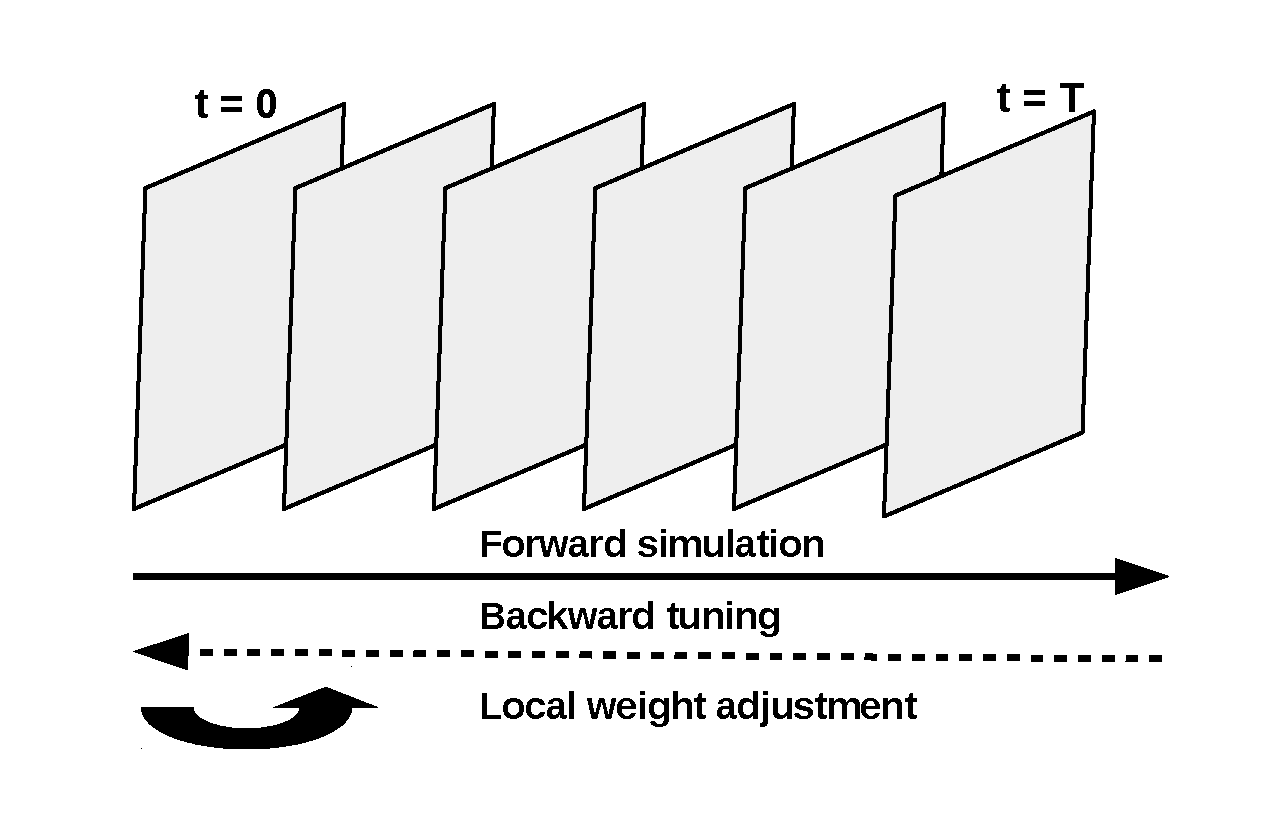
\includegraphics[width=0.8\textwidth]{img/estimation-algo}
  \caption{The algorithmic structure of the estimation algorithm: A forward simulation yields the current criterion value, while the backward tuning allows us to obtain the 2nd order and 1st order local weight adjustment elements. The algorithm can be implemented in a complete distributed framework.}
  \label{estimation-algo}
\end{figure}

Collecting the previous steps the final iterative weight adjustment writes\begin{quotation}{\small 
\noindent -1- Perform a forward simulation and a backward tuning, calculating the 1st order gradient and 2nd order elements during the backward estimation.
\\\hspace{0.5cm} -2.a- Perform a 2nd order weight adjustment.
\\\hspace{0.5cm} -2.b- If it fails, attempt to perform a 1st order weight adjustment.
\\-3- Repeat -1- unless steps -2.b- fails.
}\end{quotation}

The 2nd order adjustment also uses a line search, because our experimental observation is that the 2nd order estimation tends to overestimate the local minimum. The 2nd order adjustment is not performed if the connectivity of the network is too high since it has a cubic cost.

Though the algorithm can be implemented in a complete distributed framework, in this preliminary study, the 2nd or 1st order adjustment is global, in order to limit the number of iteration on a simple sequential machine. The complete algorithmic structure is schematized in Fig.~\ref{estimation-algo}.


\clearpage
